\section{Application}

\subsection{Lancement de l'application}


	\begin{frame}
	\frametitle{Application}
	\framesubtitle{Chargement de l'application}
	
	
	\begin{center}
		\begin{tabular}{cc}
			\begin{minipage}{8cm}
				Premier chargement:
				\begin{enumerate}
					\item Création de la base de données
					\item Récupération de toutes les ressources dans le fichier XML
					\item Instanciation des objets grâce aux ressources récupérées
					\item Copie des cartes dans le répertoire d'installation du téléphone
					\item Initialisation  de la base de données
					\item Affichage de la page de création de compte local
				\end{enumerate}
			\end{minipage} &
			\begin{minipage}{4cm}
				 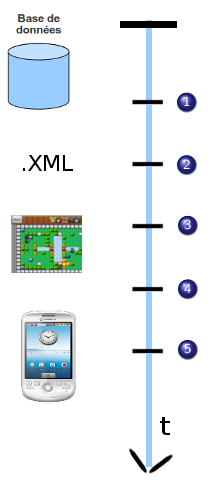
\includegraphics[scale=0.35]{img/sequence_demarrage.png}
			\end{minipage}\\
		\end{tabular}
	\end{center}

	
	\end{frame}
	
	
	\begin{frame}
	\frametitle{Application}
	\framesubtitle{Chargement de l'application}
	\begin{center}
		\begin{tabular}{cc}
			\begin{minipage}{8cm}
				Chargement standard:
				\begin{enumerate}
					\item Chargement de la base de données
					\item Récupération de toutes les ressources dans le fichier XML
					\item Instanciation des objets grâce aux ressources récupérées
					\item Instanciation du dernier utilisateur
				\end{enumerate}
			\end{minipage} &
			\begin{minipage}{4cm}
				 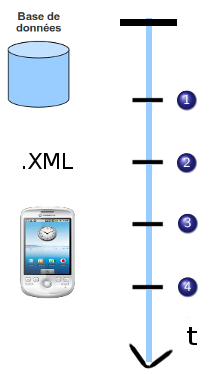
\includegraphics[scale=0.35]{img/sequence_demarrage2.png}
			\end{minipage}\\
		\end{tabular}
	\end{center}
	
	\end{frame}


	\begin{frame}
	\frametitle{Application}
	\framesubtitle{Les menus}
	
	\begin{center}
		\begin{tabular}{cc}
			\begin{minipage}{4cm}
				\begin{block}{Objectifs de conception:}
					\begin{itemize}
					  \item Interface claire
					  \item Facile d'utilisation
					  \item Navigation intuitive
					  \item Ergonomique
					\end{itemize}
				\end{block}
			\end{minipage} &
			\begin{minipage}{8cm}
				 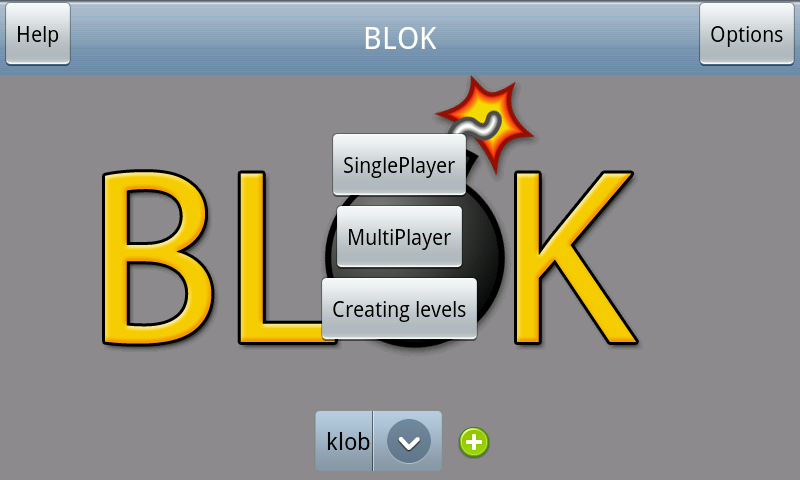
\includegraphics[scale=0.25]{img/2.png}
			\end{minipage}\\
		\end{tabular}
	\end{center}
	
		
	\end{frame}

%	\begin{frame}
%	\frametitle{Application}
%	\framesubtitle{Chargement de l'application}
%	
%	\begin{center}
%		\begin{tabular}{cc}
%			\begin{minipage}{5cm}
%				\begin{block}{Lancement}
%					\begin{itemize}
%				 		\item Initialisation des données systèmes
%			 		\end{itemize}
%				\end{block}
%			\end{minipage} &
%			\begin{minipage}{8cm}
%				 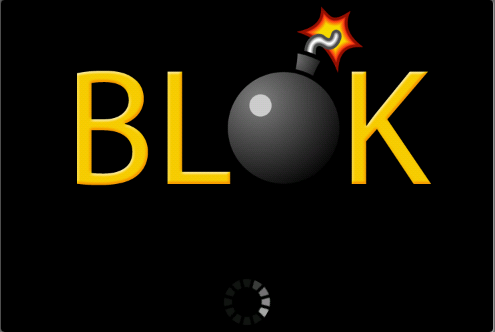
\includegraphics[scale=0.3]{img/1.png}
%			\end{minipage}\\
%		\end{tabular}
%	\end{center}
%
%		
%	
%	\end{frame}
	

	
%	\begin{frame}
%	\frametitle{Application}
%	\framesubtitle{Les menus}
%	
%		\begin{block}{Objectifs de conception:}
%			\begin{itemize}
%			  \item Interface claire
%			  \item Facile d'utilisation
%			  \item Navigation intuitive
%			  \item Ergonomique
%			\end{itemize}
%		\end{block}
%	\end{frame}
	
\subsection{Gestion des ressources}
	
	\begin{frame}
		\frametitle{Application}
		\framesubtitle{Types d'objets}
			Deux types d'objets :
			
			\begin{itemize}
				\item Non animés (tile) : une seule et unique image
					\begin{center}
						
\includegraphics[scale=0.75]{img/bloc.png}
					\end{center}
									
				\item Animés (sprite) : une sequence d'images (animation)
					
\includegraphics[scale=0.40]{img/player.png}
			\end{itemize}
	\end{frame}
	
	
	\begin{frame}
	\frametitle{Application}
	\framesubtitle{Tile mapping}

	Pourquoi ?

	\begin{enumerate}
		\item Tire ses origines des jeux des années 80
		\item Faible consommation des ressources 
		\item Performances des smartphones limitées
	\end{enumerate}
	\end{frame}

	
	\begin{frame}
		\frametitle{Application}
		\framesubtitle{Tile Mapping}		
		
		Principe :
		
		 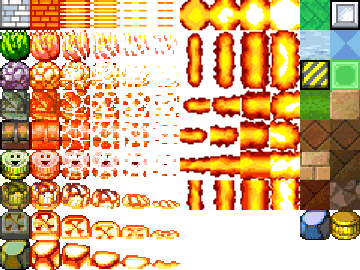
\includegraphics[scale=0.45]{img/objects.png}

	\end{frame}
	
		\begin{frame}
		\frametitle{Application}
		\framesubtitle{Gestion des ressources}
		
		XML
		\begin{itemize}
			\item Code portable
			\item Syntaxe extensible (Générique)
			\item Ajout/suppression d'éléments facile
		\end{itemize}
		
%		\begin{tiny}
%				\lstset{tabsize=1, frame=shadowbox, rulesepcolor=\color{blue}}
%		\lstinputlisting{code/objects.xml}
%		\end{tiny}


		
	\end{frame}
	
\subsection{Editeur de cartes}

	\begin{frame}
		\frametitle{Application}
		\framesubtitle{Editeur de cartes}
			\begin{center}
                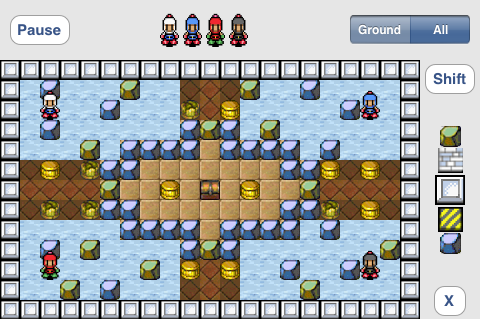
\includegraphics[width=7cm]{./img/img8.png}
            \end{center}
		\end{frame}

	\begin{frame}
		\frametitle{Application}
		\framesubtitle{Moteur de rendu (Editeur de cartes)}		
		
		Deux matrices:
		\begin{center}
			\begin{tabular}{cc}
				1^{er} niveau & 2^{ème} niveau \\
				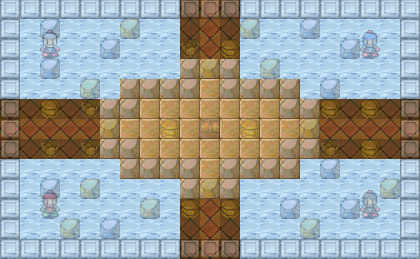
\includegraphics[width=3.5cm]{./img/img10.png} & 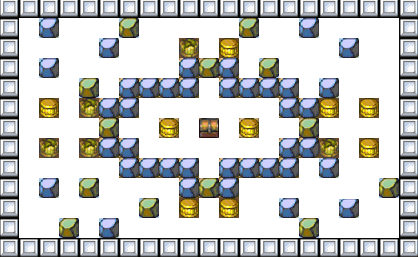
\includegraphics[width=3.5cm]{./img/img12.png} \\
				\multicolumn{2}{c}{\Downarrow} \\
				\multicolumn{2}{c}{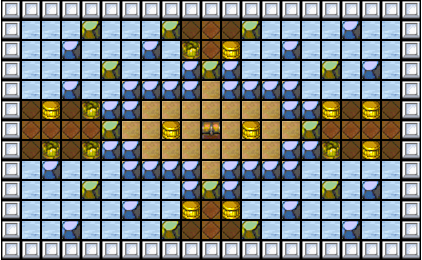
\includegraphics[width=3.5cm]{./img/img9.png}} 
			\end{tabular}
		\end{center}
	\end{frame}
	
	
%	\begin{frame}
%		\frametitle{Application}
%		\framesubtitle{Interface Utilisateur}
%		
%		\begin{center}
%        	\begin{tabular}{ll}
%                       		\begin{minipage}{4cm}
%					Différentes zones:
%                                       	\begin{itemize}
%                                   	 		\item Menu du haut
%						\item La carte
%						\item Menu droite
%                                    		\end{itemize}
%                       		\end{minipage}  &                
%                       		\begin{minipage}{5.5cm}
%                                		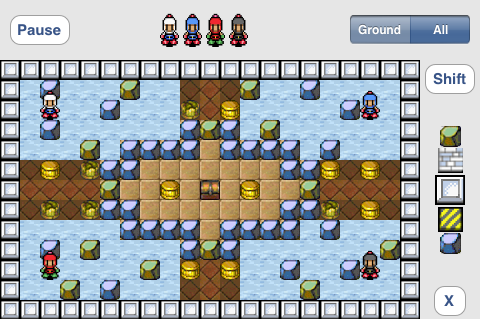
\includegraphics[width=5.5cm]{./img/img8.png}
%                       		\end{minipage}\\
%               		\end{tabular}
%               	\end{center}
%	\end{frame}
	
	
%	\begin{frame}
%		\frametitle{Application}
%		\framesubtitle{Outils}
%		
%		Deux types de listes :
%		
%		\begin{center}
%               		\begin{tabular}{p{3cm}p{3cm}}
%				Sol & Blocs \\    
%				\begin{minipage}{1cm}
%                                		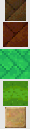
\includegraphics[scale=0.7]{./img/img4.png} \\
%				\end{minipage}
%				&
%				\begin{minipage}{1cm}
%                                		
\includegraphics[scale=0.7]{./img/img3.png} \\
%				\end{minipage}
%               		\end{tabular}
%               	\end{center}
%	\end{frame}
	
	
%	\begin{frame}
%		\frametitle{Application}
%		\framesubtitle{Possibilités finales}
%			\begin{center}
%                             	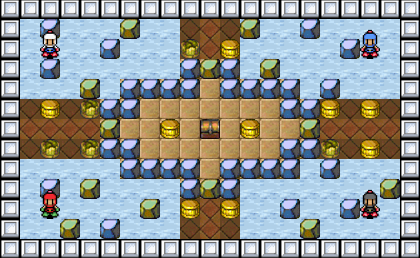
\includegraphics[width=7cm]{./img/img5.png}
%               	\end{center}
%	\end{frame}
	
%	\begin{frame}
%		\frametitle{Application}
%		\framesubtitle{Menu}
%		
%		\begin{center}
%               		\begin{tabular}{cc}
%				\begin{minipage}{3cm}
%                                       	\begin{itemize}
%                                   	 		\item Reprendre
%						\item Sauvegarder
%						\item Réinitialiser
%						\item Quitter
%                                    		\end{itemize}
%                       		\end{minipage}
%				&
%				\begin{minipage}{6cm}
%					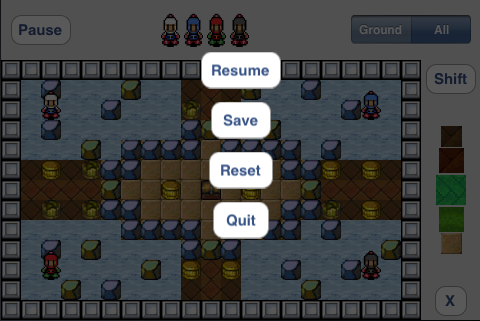
\includegraphics[width=6cm]{./img/img11.png}
%				\end{minipage}
%               		\end{tabular}
%               	\end{center}
%	\end{frame}
%
%\subsection{Jeu}
%	
%	\begin{frame}
%	\frametitle{Application}
%	\framesubtitle{Création d'une partie solitaire}
%	
%		\begin{tabular}{cc}
%			\begin{minipage}{5cm}
%				Création d'une partie solitaire
%				\begin{enumerate}
%					\item Choix de la carte
%					\item Type de la partie
%					\item Difficulté des ennemis
%					\item Nombre d'ennemis
%					\item Temps de la partie
%					\item Retourner à l'écran d'accueil
%					\item Créer la partie
%				\end{enumerate}
%			\end{minipage} &
%			\begin{minipage}{7cm}
%				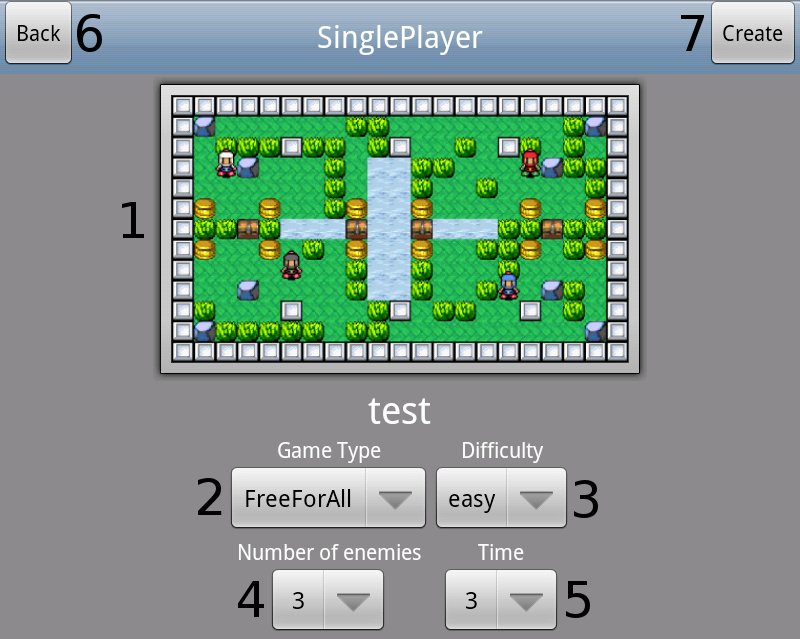
\includegraphics[width=6cm]{img/singleplayerbis.png} 
%			\end{minipage}\\
%		\end{tabular}
%	
%	\end{frame}

\subsection{Jeu}

	\begin{frame}
		\frametitle{Application}
		\framesubtitle{Jeu}
			\begin{center}
                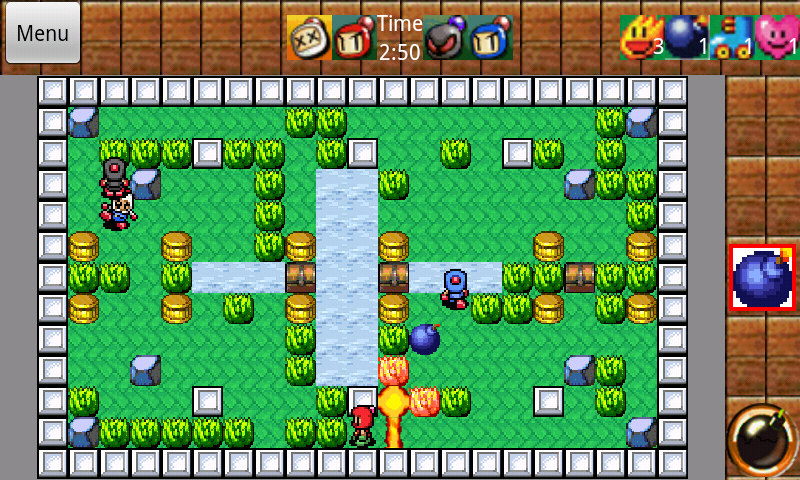
\includegraphics[width=7cm]{./img/game.png}
            \end{center}
		\end{frame}

	\begin{frame}
	\frametitle{Application}
	\framesubtitle{Moteur de rendu (Jeu)}
	
	\begin{tabular}{ccccc}
		Bitmap d'objets
		&
		&
		Table de hashage
		&
		&
		Resultat
		\\
		inanimés
		&
		&
		d'objets animés
		&
		&
		\\
		&
		&
		&
		&
		\\
		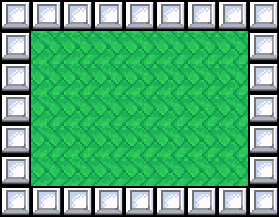
\includegraphics[width=25mm]{img/bitmap.png}
		&
		+
		&		
		\animategraphics[autoplay,loop,height=1cm]{8}{img/block_}{1}{15}
		&
		=
		&
		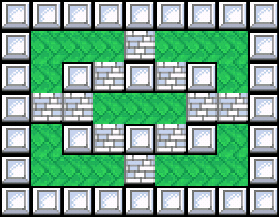
\includegraphics[width=25mm]{img/map.png}
	\end{tabular}
	
	\end{frame}
	
	
	
	\begin{frame}
	\frametitle{Application}
	\framesubtitle{Moteurs de rendu}

		Complexité en nombre d'objets à afficher \\
		
		\begin{center}
				\begin{tabular}{|c|c|c|} \hline
				  & Editeur de carte & Jeu    \\\hline 
				Meilleur des cas & 337 & 1    \\\hline
				Pire des cas     & 534 & 198  \\\hline		
				\end{tabular}
			\end{center}

	\end{frame}
	
	
	\begin{frame}
	\frametitle{Application}
	\framesubtitle{Moteur Physique}
	Carte des colisions :
	\begin{center}
		\animategraphics[controls, autoplay,loop,scale=0.3]{0.5}{img/mapcolision_}{1}{2}
	\end{center}
	\end{frame}

	\begin{frame}
	\frametitle{Application}
	\framesubtitle{Intelligence artificielle}
	
		\begin{tabular}{cc}
			\begin{minipage}{4cm}
				Niveaux de difficulté
				\begin{enumerate}
					\item Facile
					\item Moyen
					\item Difficile
				\end{enumerate}
			\end{minipage} &
			\begin{minipage}{6cm}
				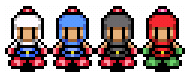
\includegraphics[width=6cm]{img/bots.png} 
			\end{minipage}\\
		\end{tabular}
	
	\end{frame}
	
	\begin{frame}
	\frametitle{Application}
	\framesubtitle{Pathfinding}
	
		\begin{tabular}{cc}
			\begin{minipage}{5cm}
				Algorithme A*
				\begin{enumerate}
					\item Heuristique (de Manatan)
					\item Coût de deplacement
					\item Premier chemin trouvé
					\item Rapidité (Dijkstra)
				\end{enumerate}
			\end{minipage} &
			\begin{minipage}{5cm}
				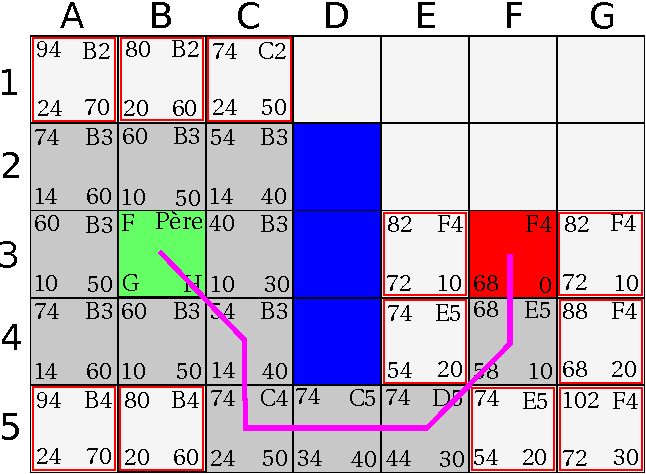
\includegraphics[width=6cm]{img/astar.png} 
			\end{minipage}\\
		\end{tabular}
	
	\end{frame}
	
	\begin{frame}
	\frametitle{Application}
	\framesubtitle{Pathfinding}
	
		\begin{tabular}{cc}
			\begin{minipage}{5cm}
				Algorithme de parcours en largeur
				\begin{enumerate}
					\item Pas de case d'arrivée nécessaire
					\item Tous les chemins possibles
					\item Premier chemin trouvé
					\item Rapidité
				\end{enumerate}
			\end{minipage} &
			\begin{minipage}{5cm}
							\begin{center}
				\animategraphics[autoplay,loop,scale=0.5]{1}{img/largeur_}{1}{4}
			\end{center}
			\end{minipage}\\
		\end{tabular}	
	
	\end{frame}
	
\subsection{Reseau}

\begin{frame}
\frametitle{Application}
\framesubtitle{Outils}
	\begin{center}
		\begin{tabular}{cc}
			\begin{minipage}{7cm}
			
			
				\begin{itemize}
				  \item Servlets
				  \item Serveur d'application
				  \item JSON
				  \item MySQL
				\end{itemize}

			
			\end{minipage}&
			
			\begin{minipage}{4cm}
				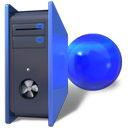
\includegraphics[scale=0.5]{img/serveur2.png} 
			\end{minipage}\\
				
			\end{tabular}
			
			\begin{block}{Remarque: }
				\begin{itemize}
				  \item Pas de moteurs de rendu
				  \item Pas d'intelligence artificielle
				  \item Moteur physique
				\end{itemize}
			\end{block}
			
			
	\end{center}
			
\end{frame}

\begin{frame}
\frametitle{Application}
\framesubtitle{Principe}

	Schéma de fonctionnement:

	\begin{center}
		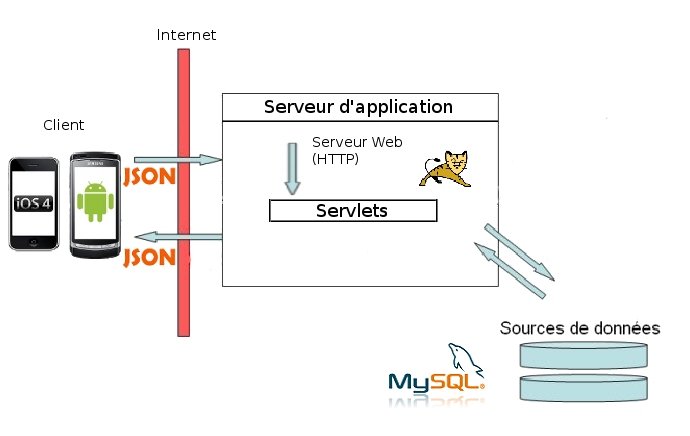
\includegraphics[width=9.4cm]{img/4.png} 
	\end{center}
	

\end{frame}

\begin{frame}
\frametitle{Application}
\framesubtitle{Exemple}

	\begin{center}
			
	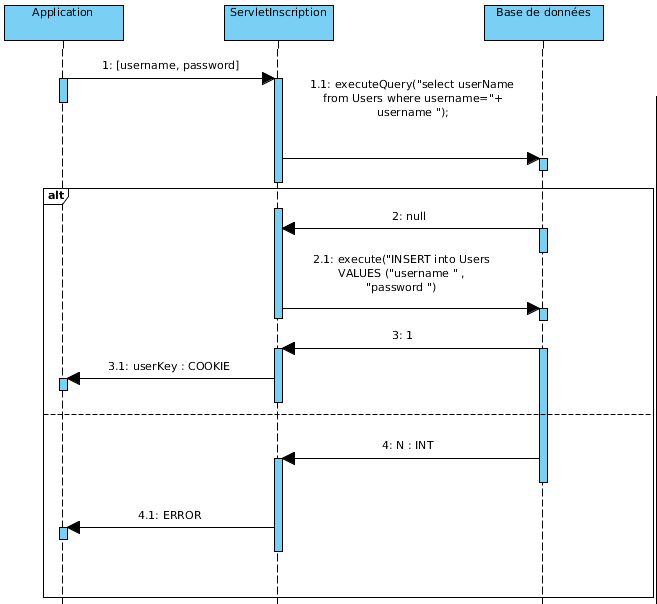
\includegraphics[scale=0.3]{img/sequence.png} 
	
	\end{center}
	

\end{frame}


\begin{frame}
\frametitle{Application}
\framesubtitle{Modélisation}

	\begin{center}
			
	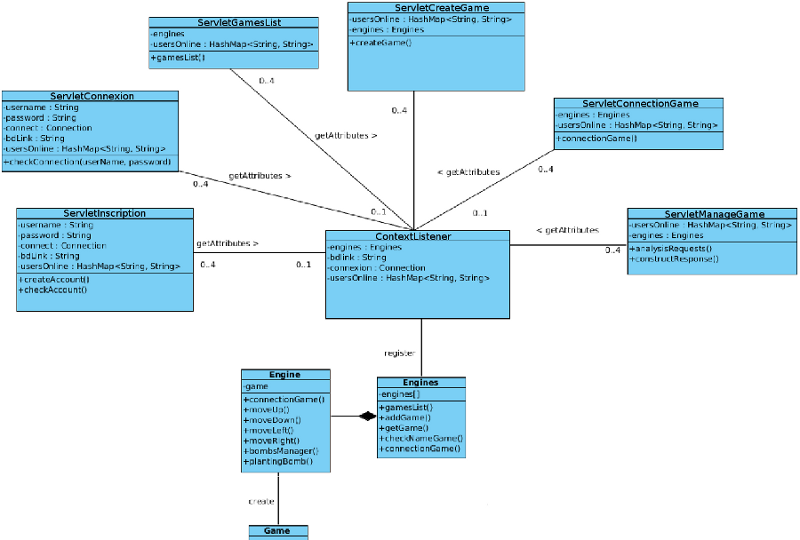
\includegraphics[width=10cm]{img/serveur.png} 
		
	\end{center}
	

\end{frame}
